\documentclass[]{report}
\usepackage[utf8]{inputenc}
\usepackage[margin=1in]{geometry}
\usepackage{graphicx}
\usepackage[backend=biber, style=apa]{biblatex}
\usepackage{csquotes}
 
\addbibresource{"uwam.bib"}
 
\author{Chen, Henry 22703907}
\title{Lithium Ion Battery Management by Texas Instruments}
 
\begin{document}
\maketitle

\chapter{Introducing the Li-Ion Battery}
Li-Ion batteries are dense power storage solutions that require precision electronics for monitoring for proper function. Li-Ion batteries also retain charge much better when compared to its Lead-Acid counterparts. Battery management is critical in the use of a Li-Ion as they are a highly volatile energy storage solution. In general, this involves (1) Precise Charge Flow Control, (2) Preventing Abuse Conditions, (3) Parameter Monitoring and (4) Charging telemetry. It is also critical to monitor each individual cell of any cell configuration and implementing redundancies in the battery pack safety system.

Typically, there is a wide range of Li-Ion cells that are suited for high peak power and high long-term use cases. It is critical to select the right battery type for the job as tradeoffs between the two attributes must be made.

\section{Li-Ion Discharge}
Typically, Li-Ion cells have a maximum cell voltage of 4.2 V however, this voltage slowly drops until the cell reaches 3.0 V. Typically, the cell's impedance can be approximated by $R=\Delta V/\Delta I$ - with higher current draws leading to higher voltage degredation. Furthermore, Li-Ion cells are highly sensitive to temperature as seen in Figure \ref{discharge_varying_temp} - at high temperatures, the cell's internal resistance decreases.

\begin{figure}[h]
    \centering
    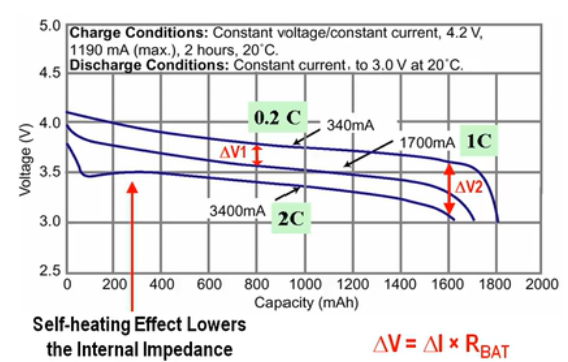
\includegraphics[width=5cm]{discharge_curve.png}
    \caption{Constant current discharge with varying current draws}
    \label{discharge_varying_current}
\end{figure}

\begin{figure}[h]
    \centering
    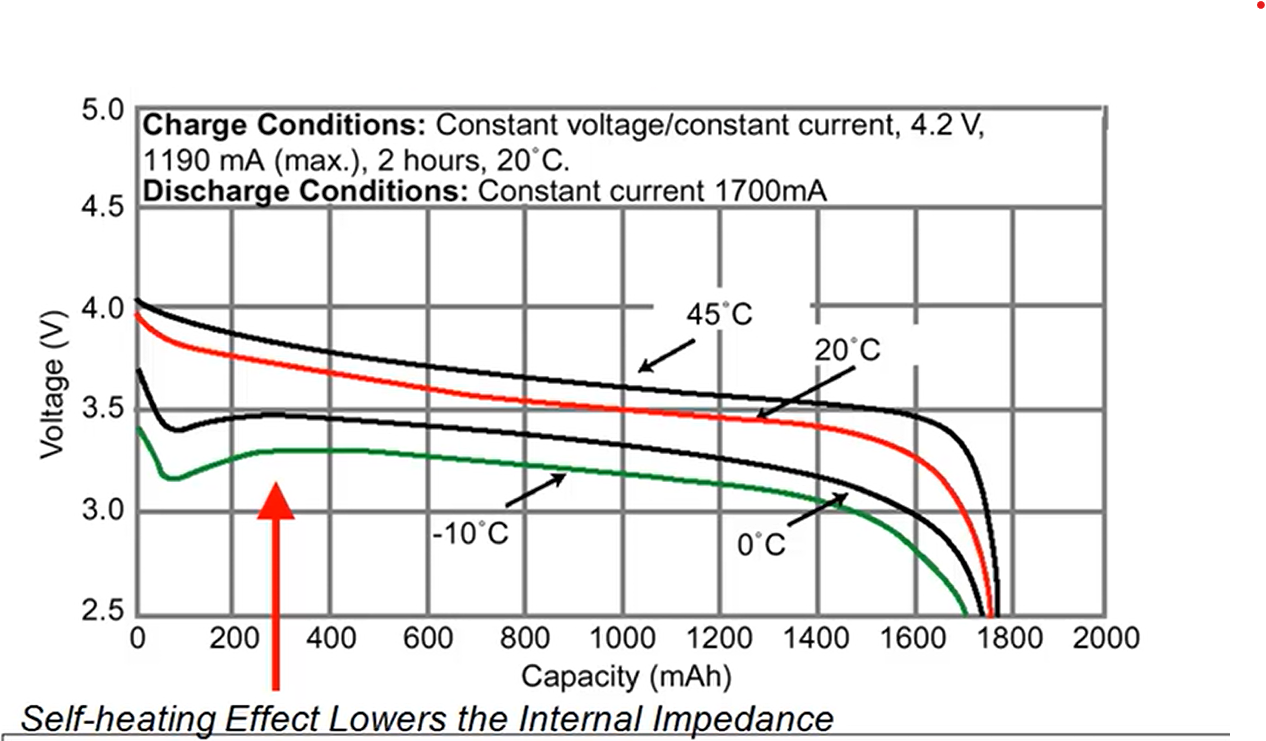
\includegraphics[width=5cm]{discharge_curve2.png}
    \caption{Constant current discharge at varying ambient temperatures}
    \label{discharge_varying_temp}
\end{figure}

\section{Cell Degredation}
As a cell is charged and discharged repeately, the internal impedance gradually increases - resulting in cells delivering less energy over its lifetime. With appropriate battery management during charging, a Li-Ion cell's degredation will be relatively performant after many cycles however, a current with 100 mA more than the cell's rated charge current will increase the gradient of the degredation curve. 

In high temperature environments, the Li-Ion cell capacity will degrade after each charge cycle. Furthermore, high current charging will also degrade the cell's capacity however (as of 2020) new cell technology may allow it to handle higher rate charging.
\end{document}